% Supplementary Figure 6 -- matched-cohort secondary modelling workflow.
%
% Step text is reproduced verbatim from the figure this replaces; only the
% drawing is new. The figure carries no title, subtitle or footnote: those
% belong to the caption in supp.tex, not to the artwork. See workflow-style.tex for the shared styling.
%
% Build with code/latex_workflow/run_all.sh (do not run pdflatex here by hand:
% the script is what puts the PDF where results/figures expects it).

\documentclass[border=6mm]{standalone}
% Shared house style for the workflow schematics.
%
% Both supplementary workflow figures are the same kind of diagram: a titled
% header, a numbered chain of steps that wraps onto a second row, and a closing
% note. Everything about how that looks lives here, so the two figure files are
% content only and cannot drift apart visually.
%
% Included by the figure files; not a standalone document.

\usepackage[T1]{fontenc}
\usepackage{lmodern}
\usepackage{tikz}
\usetikzlibrary{arrows.meta, positioning, calc}

% --- palette ---------------------------------------------------------------
% One accent per step role, dark enough to stay legible in greyscale. Header
% bars carry the accent at full strength; bodies carry an 8% tint of it.
\definecolor{wfInk}{HTML}{1F2D3D}      % body text
\definecolor{wfMuted}{HTML}{5A6B7B}    % secondary text, arrows
\definecolor{wfRule}{HTML}{C7D0D9}
\definecolor{wfSetup}{HTML}{B07D2B}    % scope-setting steps
\definecolor{wfFit}{HTML}{2E6DA4}      % fitting and prediction steps
\definecolor{wfInner}{HTML}{2E7D52}    % nested-resampling steps

% --- geometry --------------------------------------------------------------
% One box width drives everything; the header and body derive their text widths
% from it so the two nodes are exactly the same total width and align on their
% north-west corners.
\newlength{\wfBoxW}   \setlength{\wfBoxW}{52mm}
\newlength{\wfBoxH}   \setlength{\wfBoxH}{42mm}
\newlength{\wfPad}    \setlength{\wfPad}{2.6mm}
\newlength{\wfTextW}  \setlength{\wfTextW}{\dimexpr\wfBoxW-2\wfPad\relax}
\newlength{\wfHeadH}  \setlength{\wfHeadH}{7.4mm}
\newlength{\wfGapX}   \setlength{\wfGapX}{7mm}
% Five boxes and four gaps: the row-1 chain sets the canvas width, which the
% title and footnote blocks then span.
\newlength{\wfCanvasW}\setlength{\wfCanvasW}{\dimexpr 5\wfBoxW+4\wfGapX\relax}

% Resize the step boxes. The tikz styles read \wfTextW and \wfBoxH when a node
% is created, so setting these before a \wfstep call changes that box and every
% later one until it is set again. Row 2 uses wider, shorter boxes because its
% steps carry more text and there are only two of them.
\newcommand{\wfsetbox}[2]{%
  \setlength{\wfBoxW}{#1}%
  \setlength{\wfBoxH}{#2}%
  \setlength{\wfTextW}{\dimexpr\wfBoxW-2\wfPad\relax}%
}

\tikzset{
  wfbody/.style={
    draw=#1, fill=#1!8, line width=0.5pt, rounded corners=1.8pt,
    text width=\wfTextW, minimum height=\wfBoxH, inner xsep=\wfPad,
    inner ysep=0pt, align=left, anchor=north west,
  },
  wfhead/.style={
    fill=#1, text=white, text width=\wfTextW, inner xsep=\wfPad,
    inner ysep=1.9mm, align=left, anchor=north west, rounded corners=1.8pt,
    font=\sffamily\bfseries\small,
  },
  wfarrow/.style={
    -{Stealth[length=2.4mm, width=1.7mm]}, draw=wfMuted, line width=0.8pt,
  },
}

% \wfstep{<accent>}{<node name>}{<placement>}{<number>}{<title>}{<body>}
%
% The body node is drawn first and reserves the header's height at the top; the
% header bar is then laid over that reserved strip. Body text is a text width,
% so paragraphs wrap themselves and every box keeps the same footprint no matter
% how much text a step carries.
% The header height is reserved with a zero-width strut rather than \vspace*:
% inside a TikZ node with align=left the content starts in horizontal mode, so
% a leading \vspace* is applied after the first line has already been set and
% the header then covers that line. A strut forces a line box of exactly the
% header's height, whatever mode we are in.
\newcommand{\wfstep}[6]{%
  \node[wfbody=#1, #3] (#2) {%
    \rule{0pt}{\dimexpr\wfHeadH+2.2mm\relax}\par
    \color{wfInk}\sffamily\fontsize{7.6}{10}\selectfont\raggedright #6%
  };%
  \node[wfhead=#1] at (#2.north west) {#4\hspace{1.4ex}#5};%
}

% A step body is a list of short statements; \wfsep separates them.
\newcommand{\wfsep}{\par\vspace{1.5mm}}

% \wftitle{<title>}{<subtitle>}
\newcommand{\wftitle}[2]{%
  {\color{wfInk}\sffamily\bfseries\fontsize{17}{20}\selectfont #1\par}%
  \vspace{1.8mm}%
  {\color{wfMuted}\sffamily\fontsize{9}{11}\selectfont #2\par}%
  \vspace{2.8mm}%
  {\color{wfRule}\rule{\linewidth}{0.6pt}}%
}

% \wffoot{<note>}
\newcommand{\wffoot}[1]{%
  {\color{wfRule}\rule{\linewidth}{0.6pt}}\par\vspace{1.9mm}%
  {\color{wfMuted}\sffamily\itshape\fontsize{7.8}{9.6}\selectfont #1\par}%
}


\begin{document}
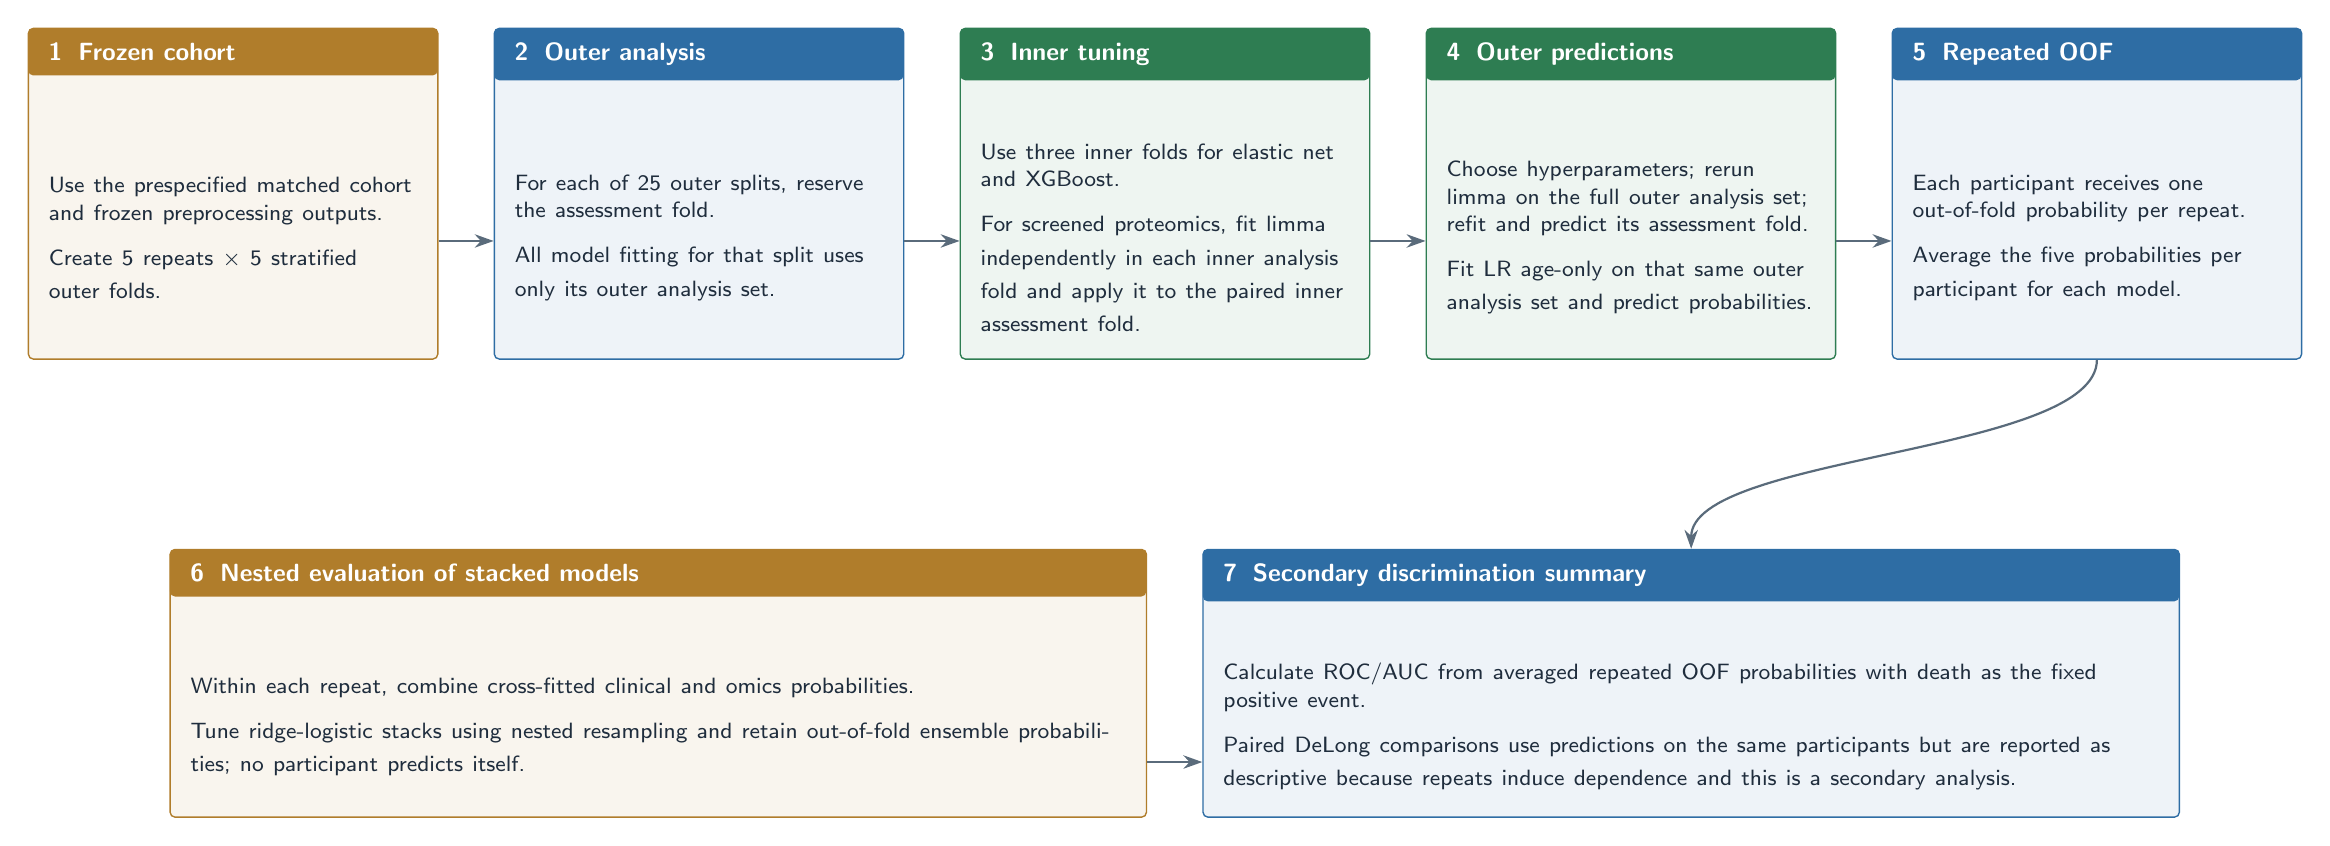
\begin{tikzpicture}[node distance=0pt]

% Row 1 -------------------------------------------------------------------
\wfstep{wfSetup}{s1}{at={(0,0)}}{1}{Frozen cohort}{%
  Use the prespecified matched cohort and frozen preprocessing outputs.\wfsep
  Create 5 repeats $\times$ 5 stratified outer folds.}

\wfstep{wfFit}{s2}{at={($(s1.north east)+(\wfGapX,0)$)}}{2}{Outer analysis}{%
  For each of 25 outer splits, reserve the assessment fold.\wfsep
  All model fitting for that split uses only its outer analysis set.}

\wfstep{wfInner}{s3}{at={($(s2.north east)+(\wfGapX,0)$)}}{3}{Inner tuning}{%
  Use three inner folds for elastic net and XGBoost.\wfsep
  For screened proteomics, fit limma independently in each inner analysis fold
  and apply it to the paired inner assessment fold.}

\wfstep{wfInner}{s4}{at={($(s3.north east)+(\wfGapX,0)$)}}{4}{Outer predictions}{%
  Choose hyperparameters; rerun limma on the full outer analysis set; refit and
  predict its assessment fold.\wfsep
  Fit LR age-only on that same outer analysis set and predict probabilities.}

\wfstep{wfFit}{s5}{at={($(s4.north east)+(\wfGapX,0)$)}}{5}{Repeated OOF}{%
  Each participant receives one out-of-fold probability per repeat.\wfsep
  Average the five probabilities per participant for each model.}

% Row 2 -------------------------------------------------------------------
% Two steps rather than five, each carrying more text: wider and shorter.
\wfsetbox{124mm}{34mm}

\wfstep{wfSetup}{s6}{at={($(s1.south west)+(18mm,-24mm)$)}}{6}{Nested evaluation of stacked models}{%
  Within each repeat, combine cross-fitted clinical and omics probabilities.\wfsep
  Tune ridge-logistic stacks using nested resampling and retain out-of-fold
  ensemble probabilities; no participant predicts itself.}

\wfstep{wfFit}{s7}{at={($(s6.north east)+(\wfGapX,0)$)}}{7}{Secondary discrimination summary}{%
  Calculate ROC/AUC from averaged repeated OOF probabilities with death as the
  fixed positive event.\wfsep
  Paired DeLong comparisons use predictions on the same participants but are
  reported as descriptive because repeats induce dependence and this is a
  secondary analysis.}

% Flow --------------------------------------------------------------------
\foreach \a/\b in {s1/s2, s2/s3, s3/s4, s4/s5}{%
  \draw[wfarrow] ($(\a.east)+(0,-6mm)$) -- ($(\b.west)+(0,-6mm)$);
}
\draw[wfarrow] (s5.south) .. controls ($(s5.south)+(0,-12mm)$) and
  ($(s7.north)+(0,12mm)$) .. (s7.north);
\draw[wfarrow] ($(s6.east)+(0,-10mm)$) -- ($(s7.west)+(0,-10mm)$);

\end{tikzpicture}
\end{document}
